\section{Analisi dei dati}\label{sec:analisi}

Il dataset \cite{datasetarticle} contiene 165633 sample e 19 features, dopo una veloce analisi dei dati è stata fatta una conversione di tipo, da stringa a tipo numerico, in particolare la feature \textit{body\_mass\_index} e la feature \textit{how\_tall\_in\_meters} sono state convertite da stringhe a tipo numerico. Inoltre la feature \textit{z4}, che rappresenta la coordinata z del quarto accelerometro, avendo un sample con un valore non numerico è stata convertita in modo forzato in tipo numerico, trasformando il valore errato in NaN, dopodichè è stato scelto di eliminare il sample con questo valore dal dataset.  Nel resto dei dati non sono presenti valori nulli o anomali.
Il dataset risulta sbilanciato per quanto riguarda la feature target, chiamata \textit{class}, come si vede dalla figura \ref{fig:bilanciamento} infatti sono presenti più samples per le classi \textit{sitting}, \textit{standing} e \textit{walking}. Quindi sarà necessario stratificare durante lo splitting del dataset e utilizzare delle metriche opportune, come l'accuracy bilanciata invece dell'accuracy semplice.

\begin{figure}[h]
    \centering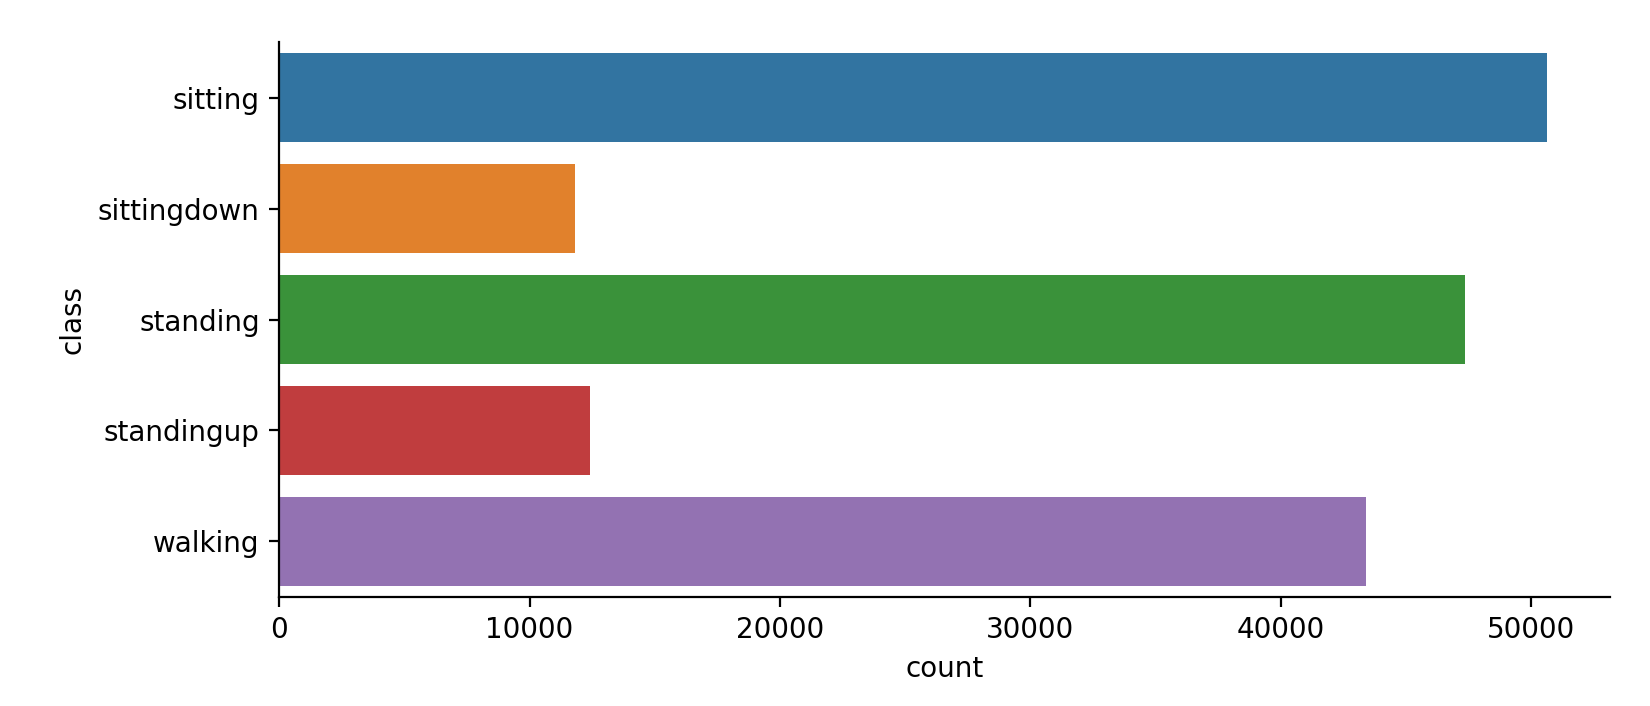
\includegraphics[width=0.8\linewidth]{bilanciamento}
    \caption{Bilanciamento della variabile target.}
    \label{fig:bilanciamento}
\end{figure}

Come si vede invece dalla figura \ref{fig:bilanciamentousers} i sample raccolti per ogni soggetto dell'esperimento sono bilanciati per tre soggetti mentre sono in misura minore per il soggetto \textit{jose\_carlos}. Dalla figura \ref{fig:classiusers} si vede invece per ogni soggetto la percentuale di sample relativi a ogni classe, e questo rispecchia il bilanciamento generale delle classi mostrato in figura \ref{fig:bilanciamento}, infatti le percentuali sono simili, in particolare le classi \textit{sittingdown} e \textit{standingup} sono presenti in misura minore.

\begin{figure}[h]
    \centering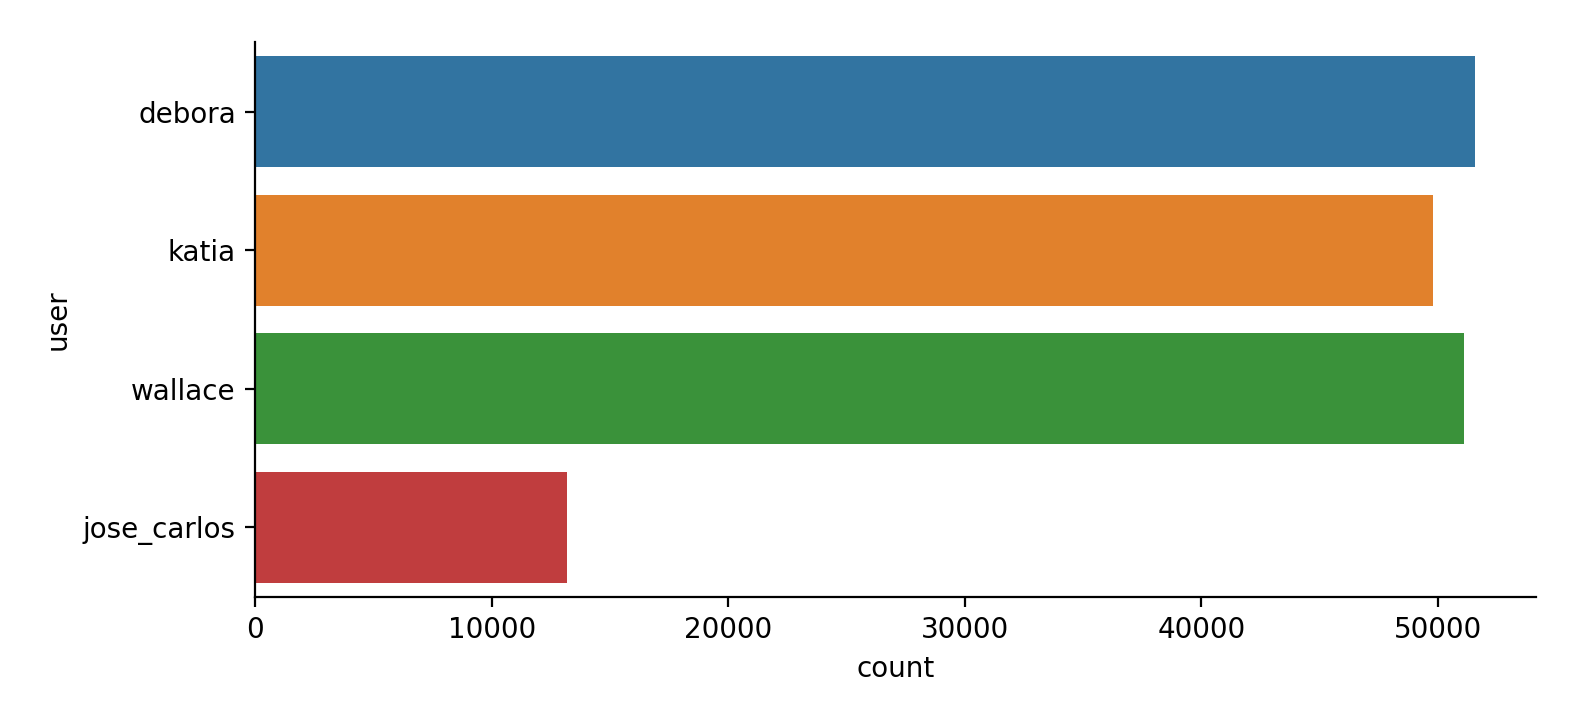
\includegraphics[width=0.5\linewidth]{bilanciamentousers}
    \caption{Bilanciamento dei dati raccolti per ogni soggetto.}
    \label{fig:bilanciamentousers}
\end{figure}

\begin{figure}[h]
    \centering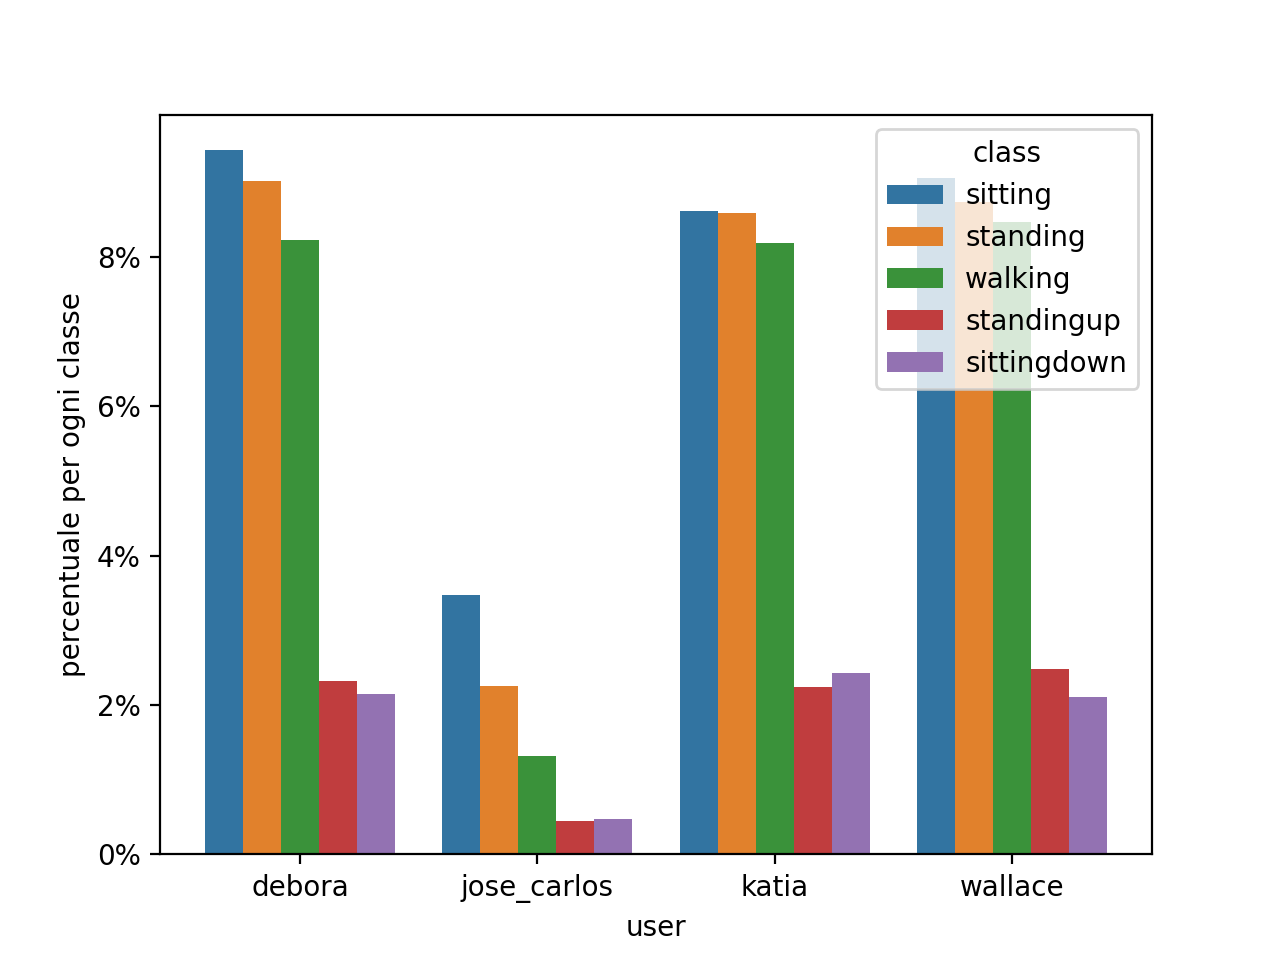
\includegraphics[width=0.5\linewidth]{divisioneclassiperuser}
    \caption{Bilanciamento delle classi per ogni soggetto.}
    \label{fig:classiusers}
\end{figure}

In figura \ref{fig:kde} sono rappresentate le distribuzioni di probabilità dei dati raccolti dall'accelerometro 2, cioè quello posto sulla coscia sinistra, classificati in base alla posizione dei soggetti. Si può notare come nel caso della classe \textit{sitting} e \textit{standing} tutte e tre le coordinate sono più concentrate nell'intorno di un unico valore, infatti la cosiddetta \textit{campana} è più stretta e alta. Questo può significare che se il valore letto è lontano dal valore di riferimento difficilmente la posizione sarà una delle due tra \textit{sitting} e \textit{standing}.

\begin{figure}[h]
    \centering
    \begin{subfigure}[t]{0.4\textwidth}
        \centering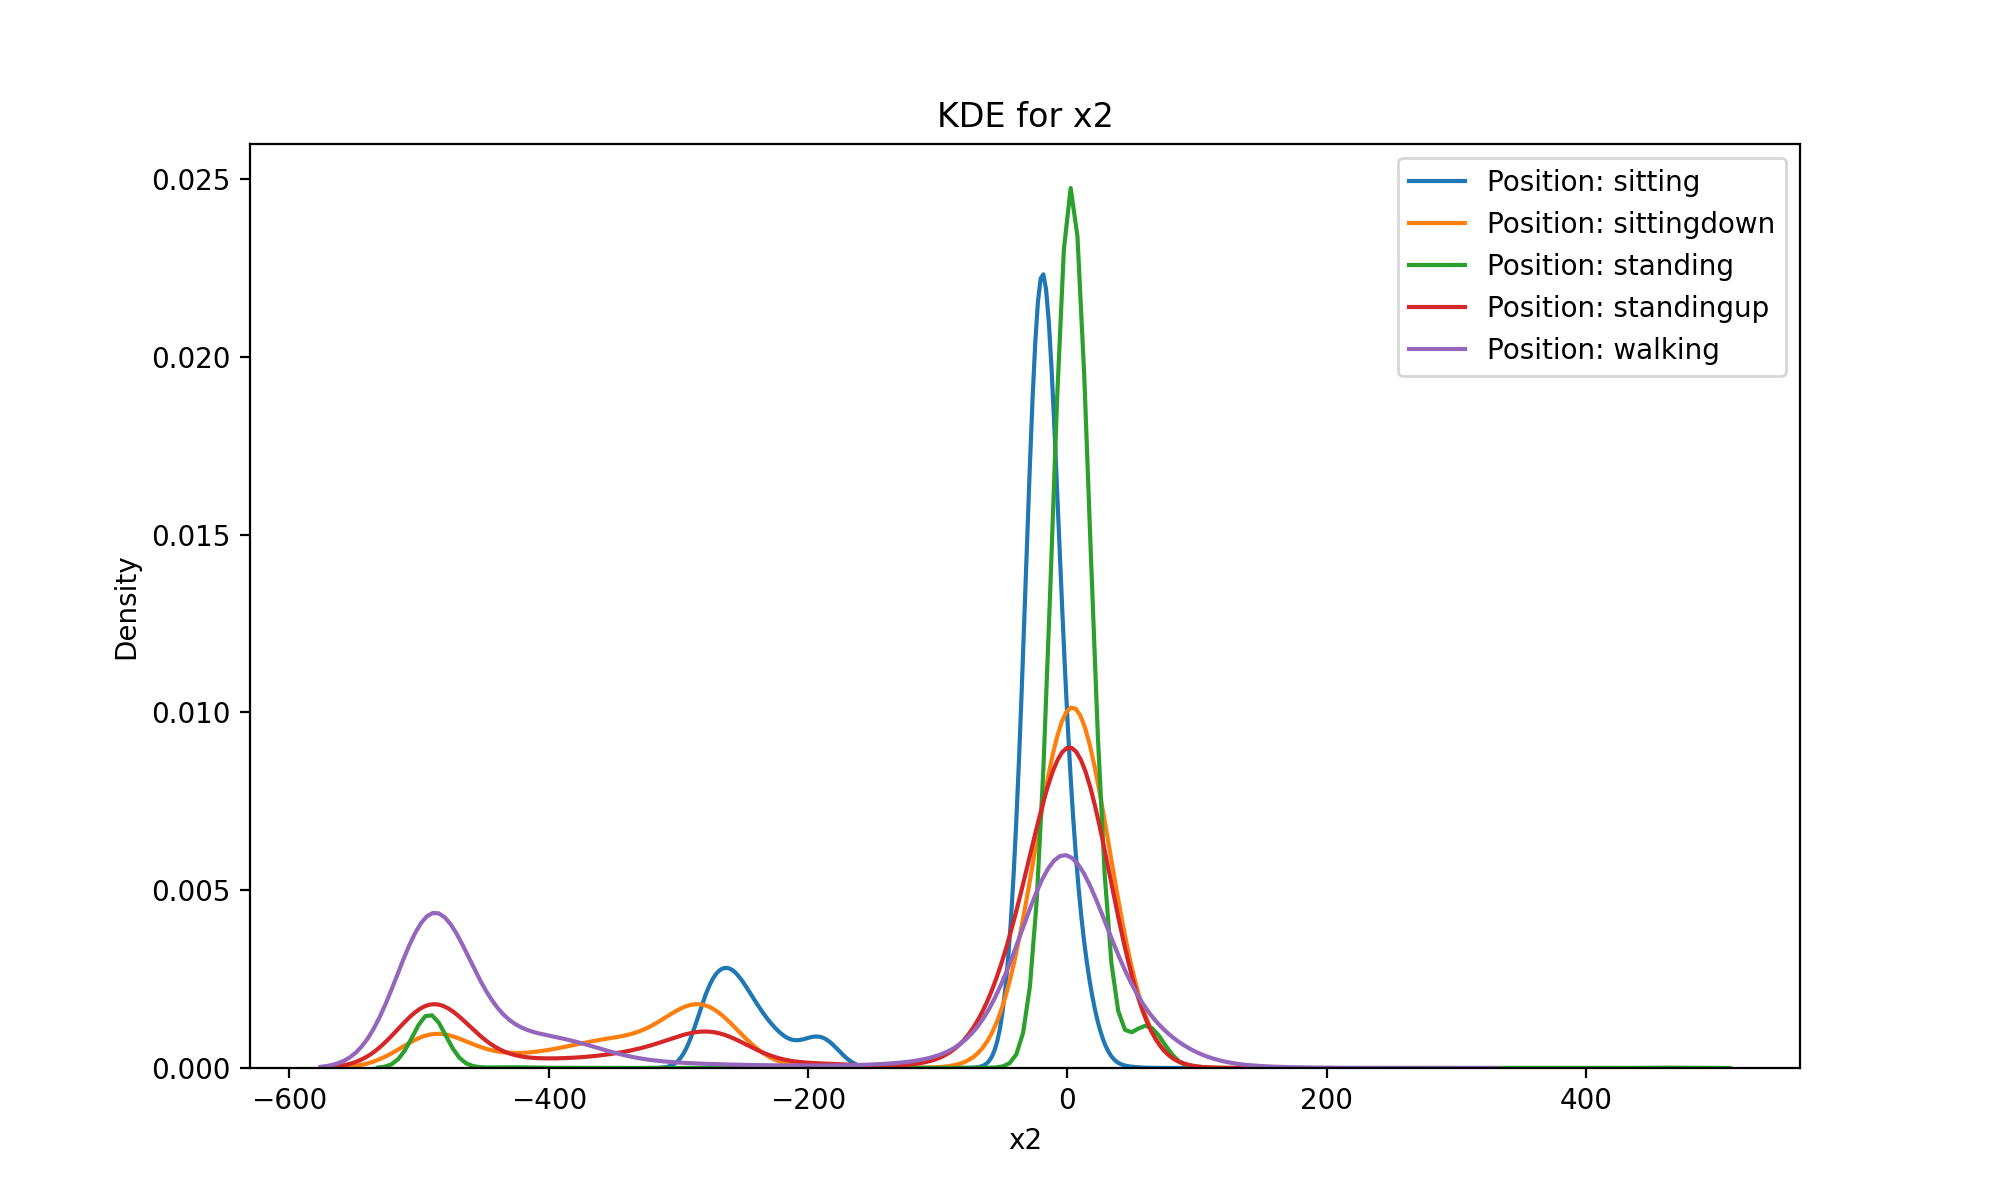
\includegraphics[width=1\linewidth]{x2}
        \caption{Distribuzione della coordinata x.}
        \label{fig:kde:x2}
    \end{subfigure}
    %
    \begin{subfigure}[t]{0.4\textwidth}
        \centering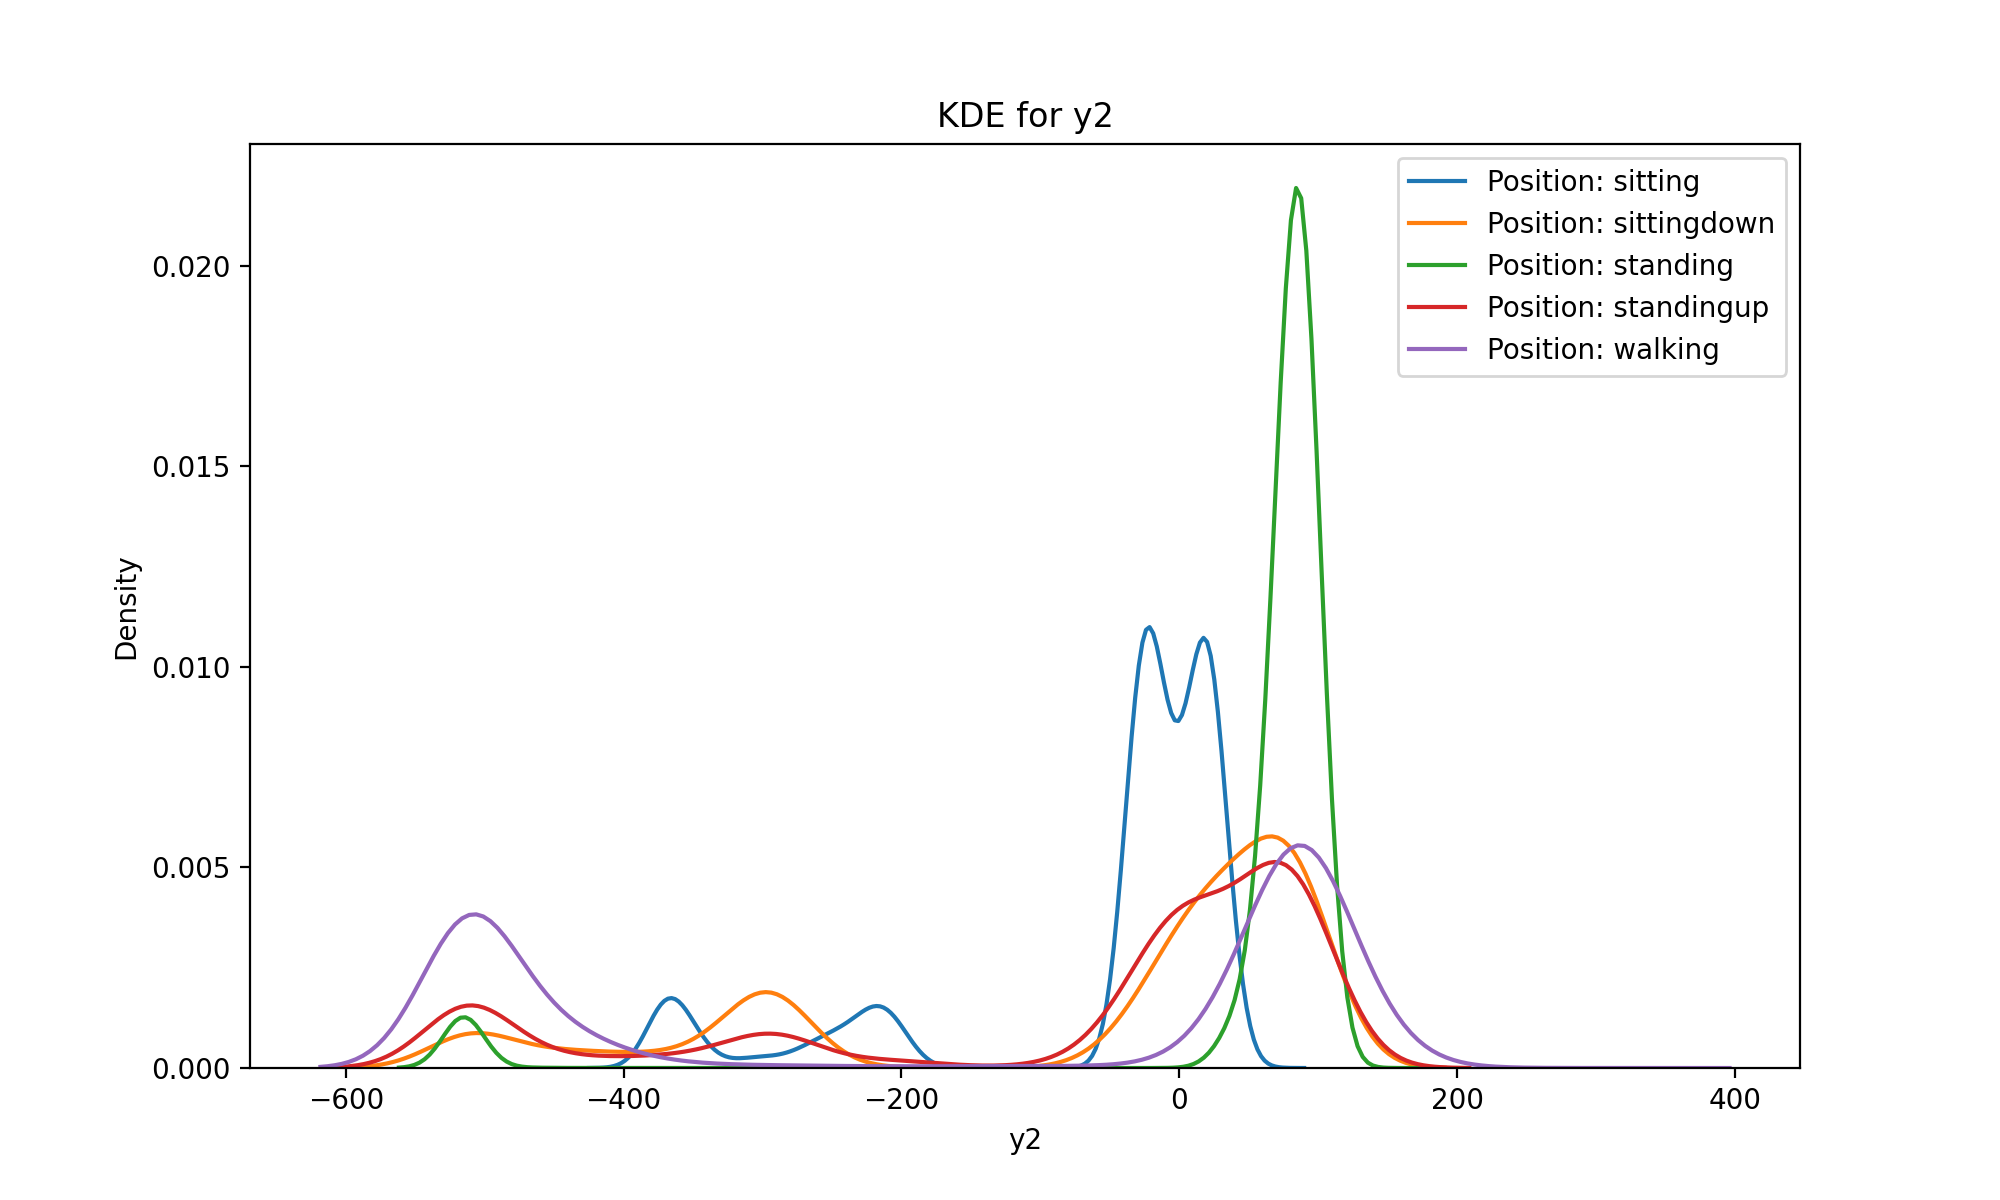
\includegraphics[width=1\linewidth]{y2}
        \caption{Distribuzione della coordinata y.}
        \label{fig:kde:y2}
    \end{subfigure}
    %
    \\
    \begin{subfigure}[t]{0.4\textwidth}
        \centering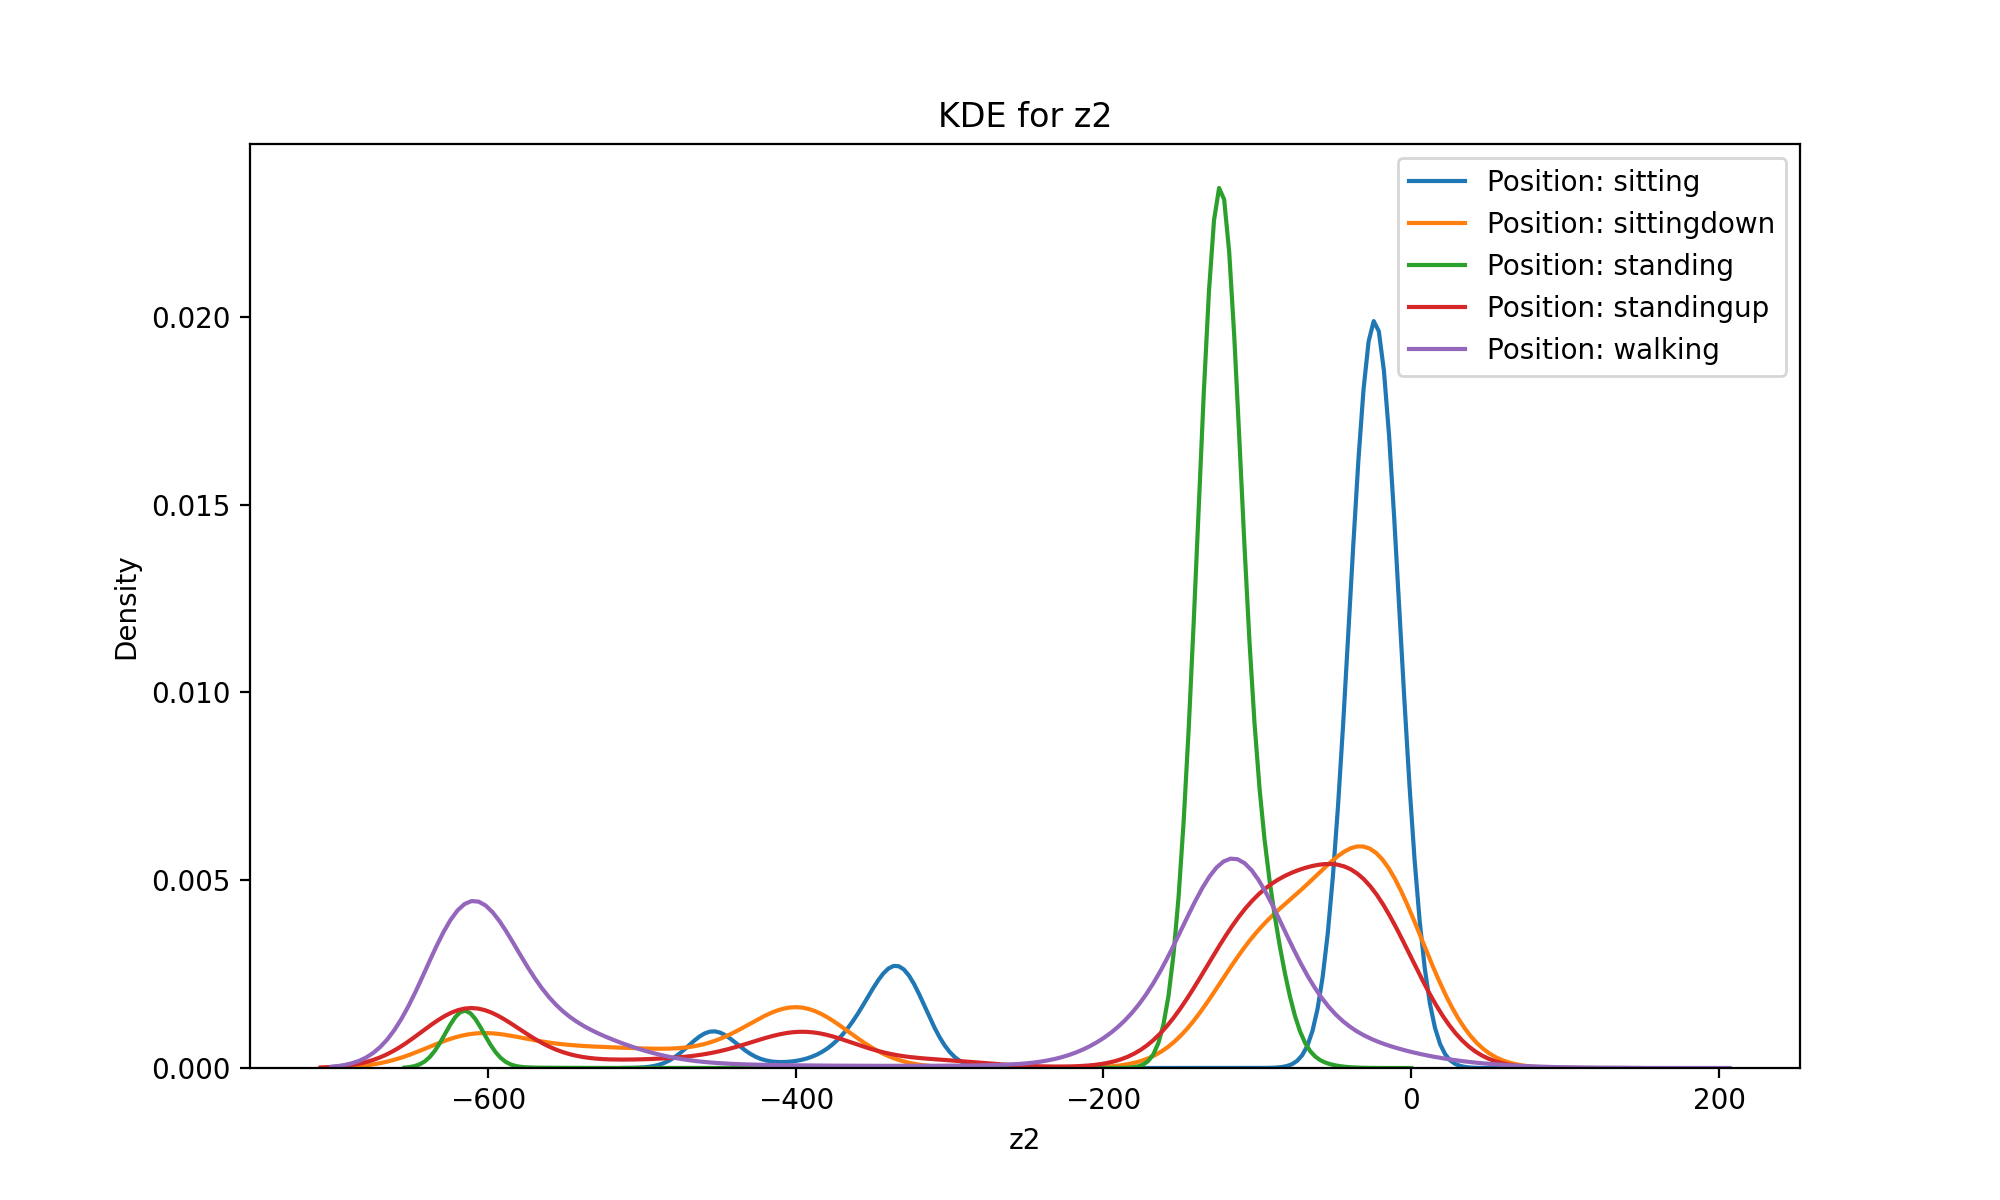
\includegraphics[width=1\linewidth]{z2}
        \caption{Distribuzione della coordinata z.}
        \label{fig:kde:z2}
    \end{subfigure}
    %
    \caption{Densità delle coordinate dell'accelerometro 2.}
    \label{fig:kde}
\end{figure}

Nella figura \ref{fig:pairplot} si vede la relazione tra le coordinate dell'accelerometro 2 e le coordinate di tutti gli accelerometri divisi per classe. Le informazioni utili che si ricavano da questo grafico sono che le coordinate dell'accelerometro 3, quello sulla caviglia destra, differiscono da quelle dell'accelerometro 2 nel caso di posizione \textit{standingup} e \textit{walking}, infatti la zona rossa, che rappresenta la posizione \textit{standingup}, assume valori minori in termini di coordinate dell'accelerometro 3. Il resto delle classi non sono distinguibili e le coordinate assumono un range di valori simile tra loro.

\begin{figure}[h]
    \centering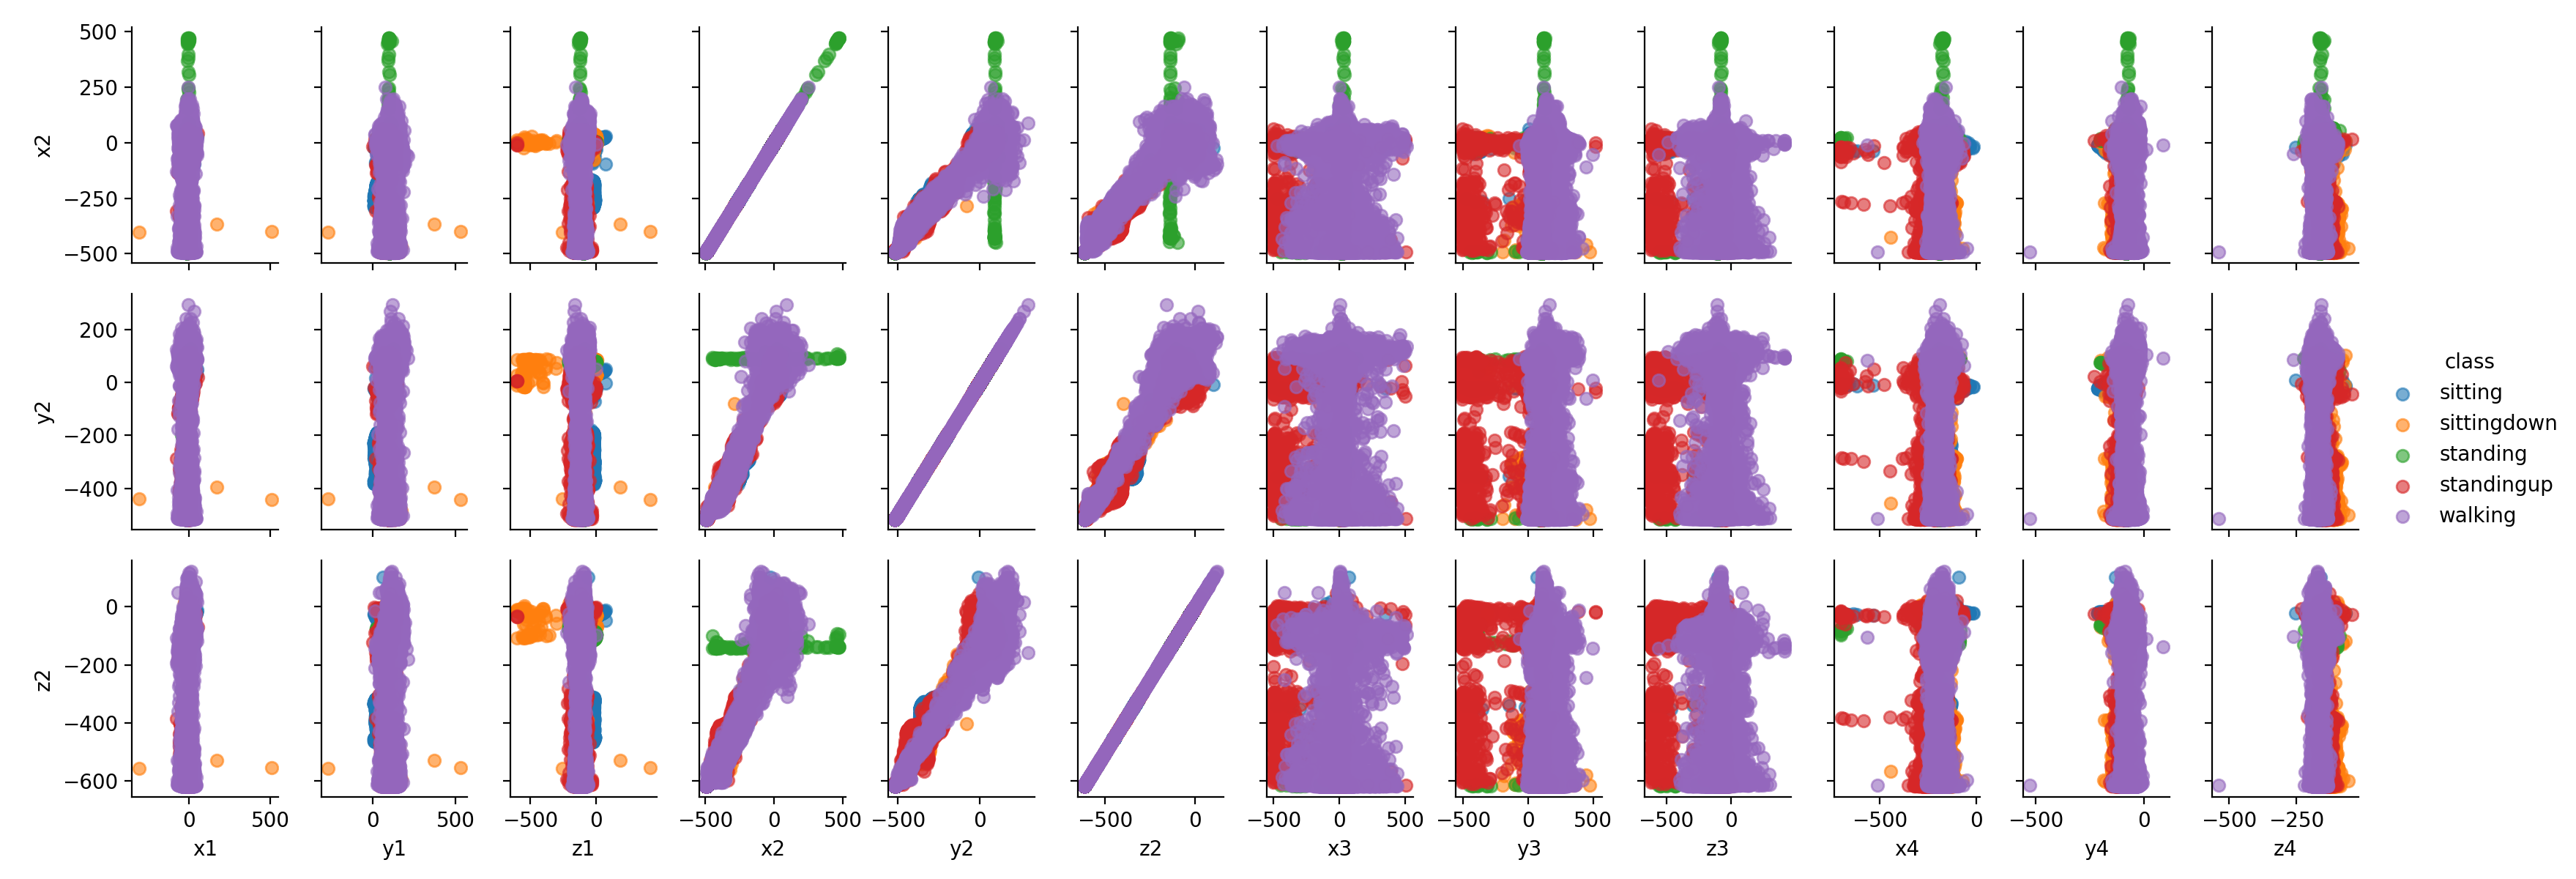
\includegraphics[width=1.0\linewidth]{pairplotacc2}
    \caption{Pairplot delle coordinate dell'accelerometro 2.}
    \label{fig:pairplot}
\end{figure}

L'accelerometro 1, quello posto sulla vita, legge delle coordinate a seconda della posizione che sono rappresentate in figura \ref{fig:scatterplot}. Come si vede dai tre grafici rappresentanti le tre coordinate, i valori non variano molto al variare della posizione, eccezion fatta per la coordinata z che diminuisce il suo valore in posizione \textit{sitting down}. Questa informazione è ragionevole, infatti la vita è la parte del corpo che cambia meno la sua posizione nello spazio al variare della postura.  Quando ci siede invece l'altezza della vita (rappresentata dalla coordinata z) si abbassa e quindi diminuisce la coordinata relativa. Inoltre dai grafici \ref{fig:scatterplot:x1}, \ref{fig:scatterplot:y1}, \ref{fig:scatterplot:z1} è possibile notare degli high leverage point presenti nei dati, cioè quei sample che differiscono dagli altri in termini di valore di una feature, in questo caso le feature \textit{x1}, \textit{y1} e \textit{z1}.

\begin{figure}[h]
    \centering
    \begin{subfigure}[t]{0.4\textwidth}
        \centering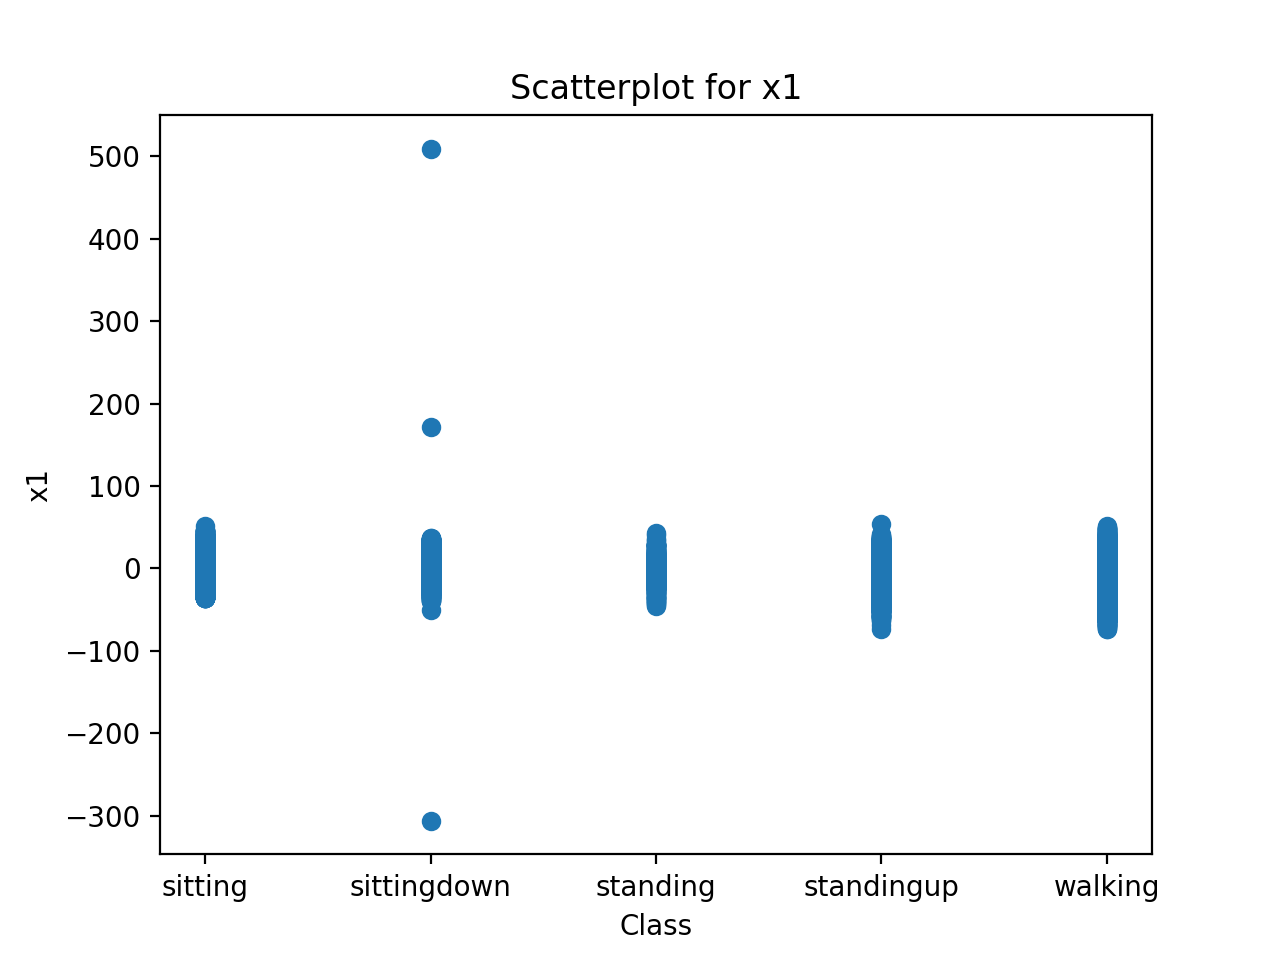
\includegraphics[width=1\linewidth]{scatx1}
        \caption{Scatterplot della coordinata x.}
        \label{fig:scatterplot:x1}
    \end{subfigure}
    %
    \begin{subfigure}[t]{0.4\textwidth}
        \centering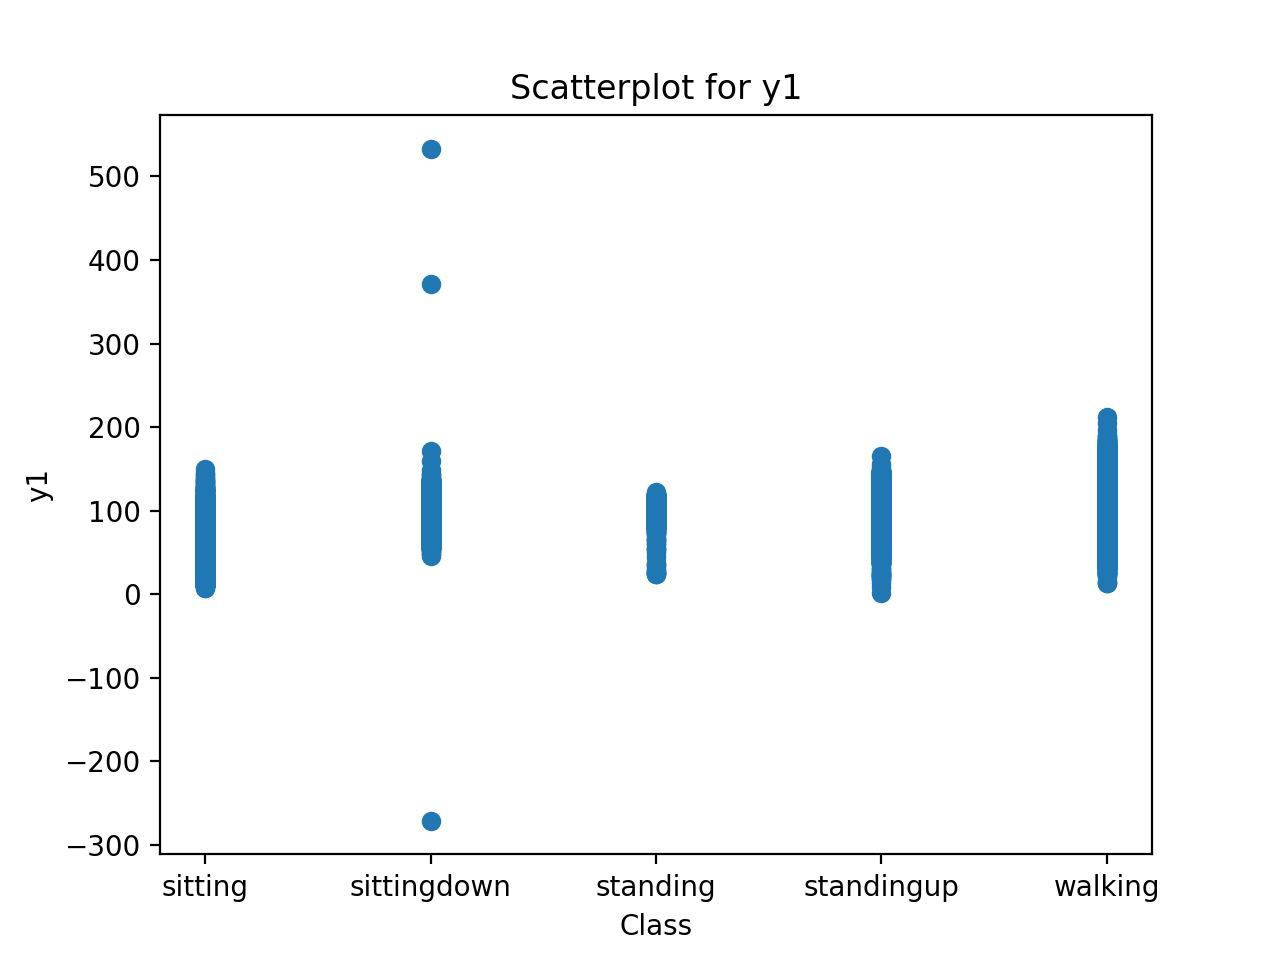
\includegraphics[width=1\linewidth]{scaty1}
        \caption{Scatterplot della coordinata y.}
        \label{fig:scatterplot:y1}
    \end{subfigure}
    %
    \\
    \begin{subfigure}[t]{0.4\textwidth}
        \centering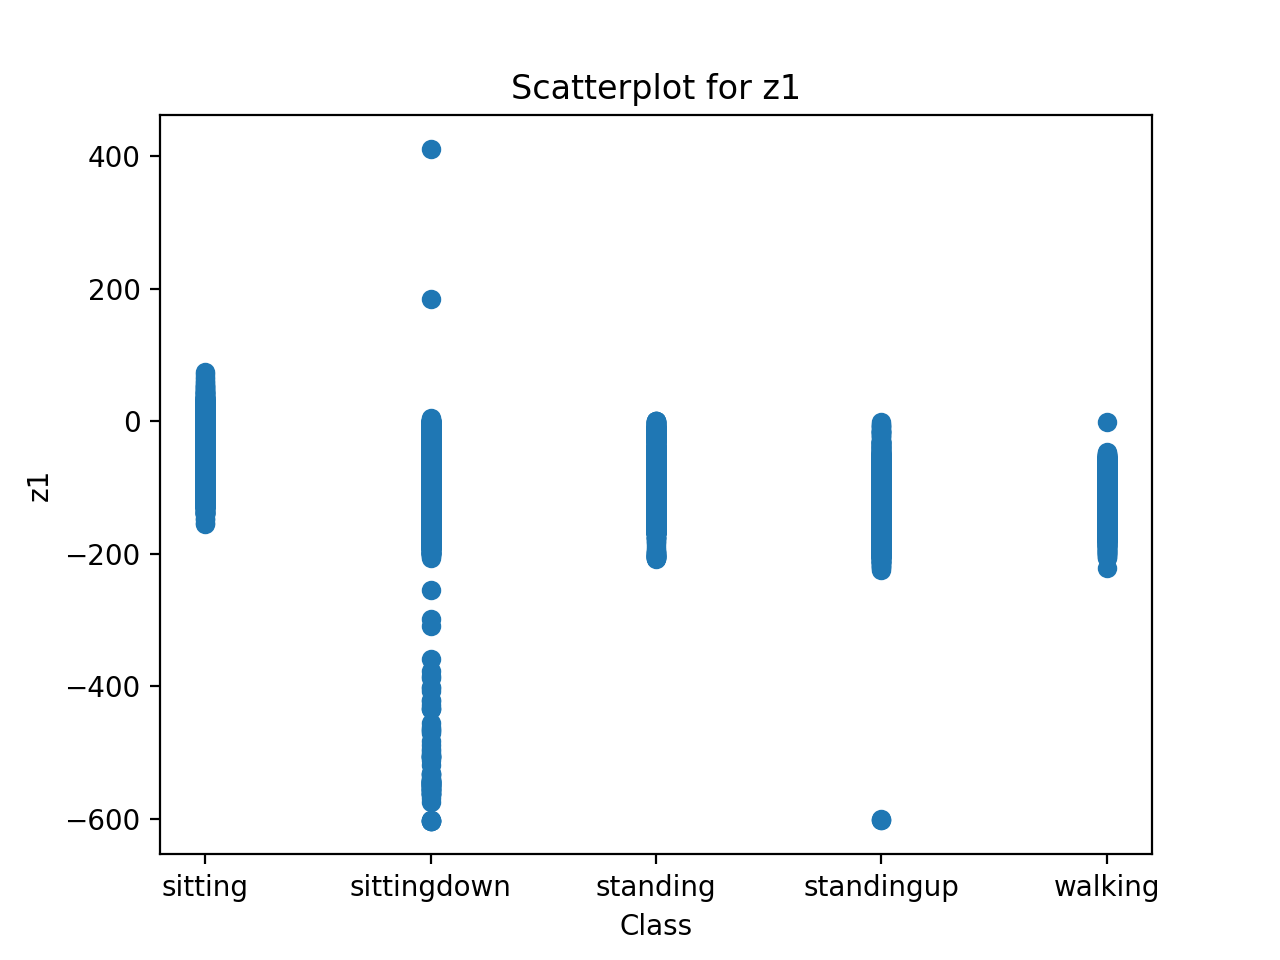
\includegraphics[width=1\linewidth]{scatz1}
        \caption{Scatterplot della coordinata z.}
        \label{fig:scatterplot:z1}
    \end{subfigure}
    %
    \caption{Scatterplot delle coordinate dell'accelerometro 1.}
    \label{fig:scatterplot}
\end{figure}

Nella fase di pre-processing delle variabili è stato fatto un encoding delle features categoriche, in particolare la feature \textit{gender} è stata trasformata con un oggetto di tipo \verb+LabelEncoder()+, che ha mappato i due possibili valori, \textit{man} e \textit{woman}, in numeri, \textit{0} e \textit{1} rispettivamente.  Inoltre è stato fatto l'encoding con lo stesso metodo anche della variabile target, \textit{class}, mappando le cinque classi con numeri da \textit{0} a \textit{4}. Dopodiché è stato effettuato il min-max-scaling alle features, che porta il valore di ogni feature tra 0 e 1, per velocizzare il training dei modelli.  Inoltre per alcuni modelli è stato deciso di fare una riduzione delle features tramite la PCA (Principal Component Analysis), che sarà però approfondita nella sezione \ref{sec:implementazione}.
Infine il criterio di splitting scelto per il dataset è stato il seguente:
\begin{itemize}
\item \textbf{training set}: 80\% del dataset originale
\item \textbf{test set}: 20\% del dataset originale
\end{itemize}
Lo splitting è stato fatto in modo stratificato in modo da effettuare la divisione mantenendo bilanciate le classi della variabile target.

In fase di cross validazione sarà poi effettuato un ulteriore splitting del training set, in validation set e development set per fare la model selection per la scelta opportuna dei parametri dei vari modelli, e la model assessment per stimare le prestazioni dei modelli. 